\subsection{Hyperledger Composer}
\label{sec:prototype_composer}
        Hyperledger Composer ist ein Framework für das Entwickeln von Blockchain-Netzwerken und dient vornehmlich als Abstraktion des Hyperledger Fabric Frameworks. 
        \medskip\\
        Fabric bietet die Möglichkeit Private- oder Consortium-Blockchainnetzwerke zu entwickeln und zu betreiben, wobei eigens konfigurierbare 
        \medskip\\
        \noindent Für die Entwicklung der Transaktionslogik von Business Networks wird die Sprache JavaScript verwendet. 
        Zusätzlich werden domainspezifische Sprachen für die Modellierung der Akteure im Netzwerk, sowie der Zugriffskontrolle und Anfragen and die Blockchcain eingesetzt.
        Als Datenbank kann LevelDB oder CouchCB verwendet werden.
        Betrieben wird die Applikation innerhalb eines Docker-Containers.
        
        \noindent Für den Prototypen relevante Eigenschaften des Hyperledger Composer Frameworks:
        \begin{itemize}[noitemsep]
            \item Ein Blockchain-Netzwerk wird im Kontext des Frameworks als ,,Business Network`` bezeichnet. 
            \item Ein Business Network besteht aus Assets, Participants, Transactions, \gls{acl}, Events (optional) und Queries (optional).
                \begin{itemize}[noitemsep]
                    \item Assets: Güter, die auf der Blockchain gespeichert sind.
                    \item Participants: Teilnehmer des Netzwerkes.
                    \item Transactions: Funktionen, die ausgeführt werden können, können Smart Contracts (Transaction Processor Functions) auslösen, welche beliebige Aktionen ausfüren können. 
                    \item Access Control Rules: legen fest, welche Teilnehmer welche Aktionen im Netzwerk ausüben dürfen. 
                        Zu vergebende Berechtigungen (CRUD
                        \!\footnote{Create, Read, Update, Delete}
                        ) beschränken sich auf Assets und Transactions und werden sequentiell in geordneter Reihenfolge ausgewertet. 
                \end{itemize}
            \item Metadaten wie Dependencies und Versionsnummern werden in einer separaten Datei (\colorbox{light-gray}{\lstinline|package.json|}) abgelegt.
            \item bei der Ausführung einer Transaktion kann gleichzeitig optional ein Smart Contract ausgeführt werden
            \item Historian registry: The historian is a specialised registry which records successful transactions, including the participants and identities that submitted them. 
            The historian stores transactions as HistorianRecord assets, which are defined in the Hyperledger Composer system namespace.
            \item Each transaction type has an associated registry storing the transactions.
        \end{itemize}
        
        \begin{figure}[H]
    		\centering
    		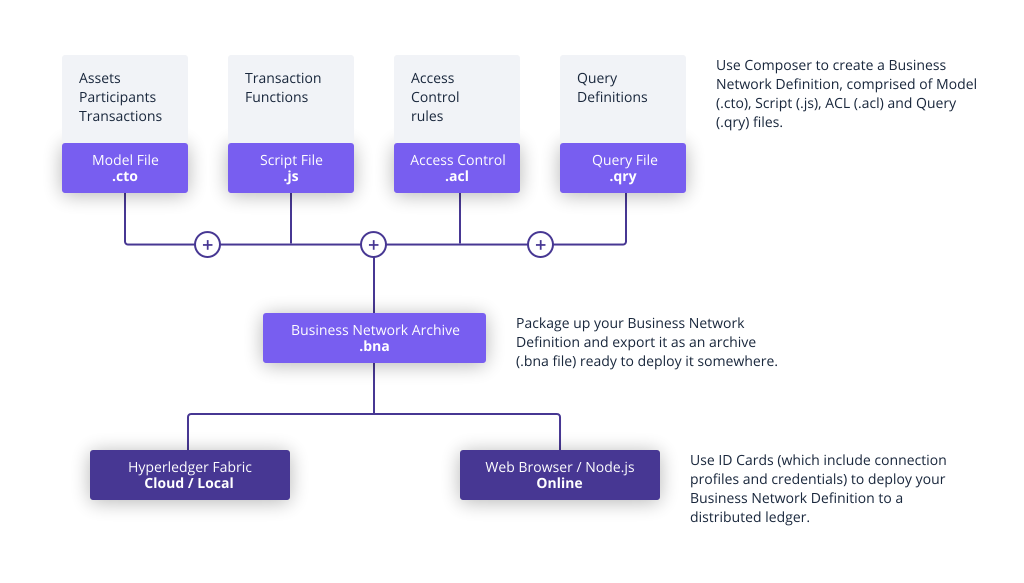
\includegraphics[width=\textwidth]{graphics/Composer-Diagram.png}
    		\caption[Bestandteile einer Hyperledger Composer-Applikation]{Bestandteile einer Hyperledger Composer-Applikation\cite{ComposerDocs}}
    		\label{fig:composer_arch}
    	\end{figure}
        
        \begin{itemize}[noitemsep]
            \item Möglichkeit eine \gls{rest}-\gls{api} pro Business Network Card mit folgenden Features zu generieren
                \begin{itemize}[noitemsep]
                    \item Nutzung von API-Keys für die Sicherung der \gls{rest}-\gls{api}
                    \item Authentifizierung via Passport auf Linux-Maschinen
                    \item ,,Explorer Test Interface``, welches automatisch generiert wird und essentiell eine Dokumentation der \gls{api} darstellt mit der zusätzlichen Möglichkeit die \gls{api}-Calls zu testen.
                    \item Key für dynamisches Logging
                    \item Event Publication via WebSocket
                    \item \gls{tls} und HTTPS für die \gls{api}
                \end{itemize}
            \item Bietet die Möglichkeit eine simple Anuglar-App zu generieren, welche letztendlich nur eine GUI-Maske für die \gls{api}-Methoden ist.
            \item Actors im Netzwerk (Peers, Orderers, Client Applications etc. haben eine digitale Identität, welche sich in einem X.509 digitalem Zeritifikat befindet.
                Die Zertifikate sind letztendlich ausschlaggebend für die Zugriffskontrolle und den Rechten, die eine Entität in dem Netzwerk erhält. 
                Zusätzlich können weitere Attribute, die zu einer Identät gehören genutzt werden (wie bspw. Organisiation, Rolle, etc.), welche eine Rolle bei der Bestimmung, welche Rechte diese Entität erhalten soll, spielen können.
            \item Zertifikate kommen von einer vertrausenswürdigen Autortität, dem \gls{msp}. 
                Gleicht einer PKI mit digitalen Zertifikaten, public/\-private Keys, CA und CRL
            \item öffentliche und private Kanäle: Nachrichtenwege, um Privatsphäre von Transaktionen und Vertraulichkeit zu gewährleisten.
                Private Kanäle sind nur für bestimmte Netzwerkmitglieder sichtbar, denen der Channel freigegeben wurde.
            \item Ordering Service: ein oder mehrere Knoten, die Transaktionen in einem Block ordnen
            \item Ledger: Blockchain + World State
            \item Deployable: Business Network Archive (bna)
            \item Historian: registry which records successful transactions, including the participants and identities that submitted them
        \end{itemize}
        
        \begin{itemize}[noitemsep]
            \item Single Organization 
            \item Membership Provider Service
        \end{itemize}
        
        Konfiguration des Frameworks
        \begin{itemize}[noitemsep]
            \item How to ensure a consistent state across all entities?...
            \item Hyperledger bietet CA für Identitäten, Authentifizierung \textrightarrow\ wie ist das bei Composer?
            \item \begin{itemize}
                \item erlaubt Sicherheitseinstellungen beim Erstellen des \gls{rest}-\gls{api}-Servers
                \item API Key
                \item Authentication mit Passport
                \item explorer Test interface ?
                \item dynamic logging
                \item event publication over websockets
                \item TLS enable/\-disable
                \item Chaincode erklären
            \end{itemize}
        \end{itemize}
    
Blockchain State Storage\\
All transactions submitted through a business network are stored on the blockchain ledger, and the current state of assets and participants are stored in the blockchain state database. The blockchain distributes the ledger and the state database across a set of peers and ensures that updates to the ledger and state database are consistent across all peers using a consensus algorithm.
\medskip
Connection Profiles\\
Hyperledger Composer uses Connection Profiles to define the system to connect to. A connection profile is a JSON document the is part of a business network card. These profiles are usually provided by the creator of the system they refer to and should be used to create business network cards in order to be able to connect to that system.
\medskip
Assets\\
Assets are tangible or intangible goods, services, or property, and are stored in registries. Assets can represent almost anything in a business network, for example, a house for sale, the sale listing, the land registry certificate for that house, and the insurance documents for that house may all be assets in one or more business networks.

Assets must have a unique identifier, but other than that, they can contain whatever properties you define. Assets may be related to other assets or participants.
\medskip
Participants\\
Participants are members of a business network. They may own assets and submit transactions. Participant types are modeled, and like assets, must have an identifier and can have any other properties as required. A participant can be mapped to one or multiple identities.
\medskip
Identities\\
An identity is a digital certificate and private key. Identities are used to transact on a business network and must be mapped to a participant in the business network. A single identity is stored in a business network card and if that identity has been mapped to a participant, it allows the user of that business network card to transact on a business network as that participant.
\medskip
Business Network cards\\
Business network cards are a combination of an identity, a connection profile, and metadata, the metadata optionally containing the name of the business network to connect to. Business network cards simplify the process of connecting to a business network, and extend the concept of an identity outside the business network to a 'wallet' of identities, each associated with a specific business network and connection profile.
\medskip
Transactions\\
Transactions are the mechanism by which participants interact with assets. This could be as simple as a participant placing a bid on a asset in an auction, or an auctioneer marking an auction closed, automatically transferring ownership of the asset to the highest bidder.
\medskip
Queries\\
Queries are used to return data about the blockchain world-state. Queries are defined within a business network, and can include variable parameters for simple customization. By using queries, data can be easily extracted from your blockchain network. Queries are sent by using the Hyperledger Composer API.
\medskip
Events\\
Events are defined in the business network definition in the same way as assets or participants. Once events have been defined, they can be emitted by transaction processor functions to indicate to external systems that something of importance has happened to the ledger. Applications can subscribe to emitted events through the composer-client API.
\medskip
Access Control\\
Business networks may contain a set of access control rules. Access control rules allow fine-grained control over what participants have access to what assets in the business network and under what conditions. The access control language is rich enough to capture sophisticated conditions declaratively, such as "only the owner of a vehicle can transfer ownership of the vehicle". Externalizing access control from transaction processor function logic makes it easier to inspect, debug, develop and maintain.
\medskip
Historian registry\\
The historian is a specialised registry which records successful transactions, including the participants and identities that submitted them. The historian stores transactions as HistorianRecord assets, which are defined in the Hyperledger Composer system namespace.
\medskip
The Hyperledger Composer Historian is a specialised registry which records successful transactions, including the participants and identities that submitted them. The historian stores transactions as HistorianRecord assets, which are defined in the Hyperledger Composer system namespace.
\medskip
An ID card (or card for short) is a collection of files that contains all the information necessary to allow a participant to connect to a business network. The card is referred to as an identity. Before it can be used, it must be issued to the user, allowing him or her to be authenticated and authorized to use the network. Cards are a very handy way of securing access to a Hyperledger Fabric network. Rather than keeping up with a password (called a secret in Hyperledger Composer terminology), you import the card into a collection of cards in the Hyperledger Fabric called a wallet. From that point on, you can just reference the card to authenticate that identi
\begin{enumerate}
    \item PeerAdmin ist für Hyperledger Instanz verantwortlich, stellt ID cards für BNA aus und entzieht dieser auch wieder, deployed business networks
    \item BNA: update network, create, issue and revoke ID cards for participants
\end{enumerate}
